\section{Single-Photon Emitters}
\label{sec:SPE}
%Bei höheren Intensitäten sollte der Dip schmaler werde, weil dann der Emitter näher an Sättigung geht und zunehmend die Lebensdauer des angeregten Zustands statt der Einstrahlphotonenrate relevant ist
%Bei 2mW angefangen zu blinken. Spektrum trotzdem gut
%Für die Spektren gegen Wellenlänge die Fläche drunter integrieren und gegen Leistung plotten

\subsection{Execution}

\begin{figure}[H]
    \centering
    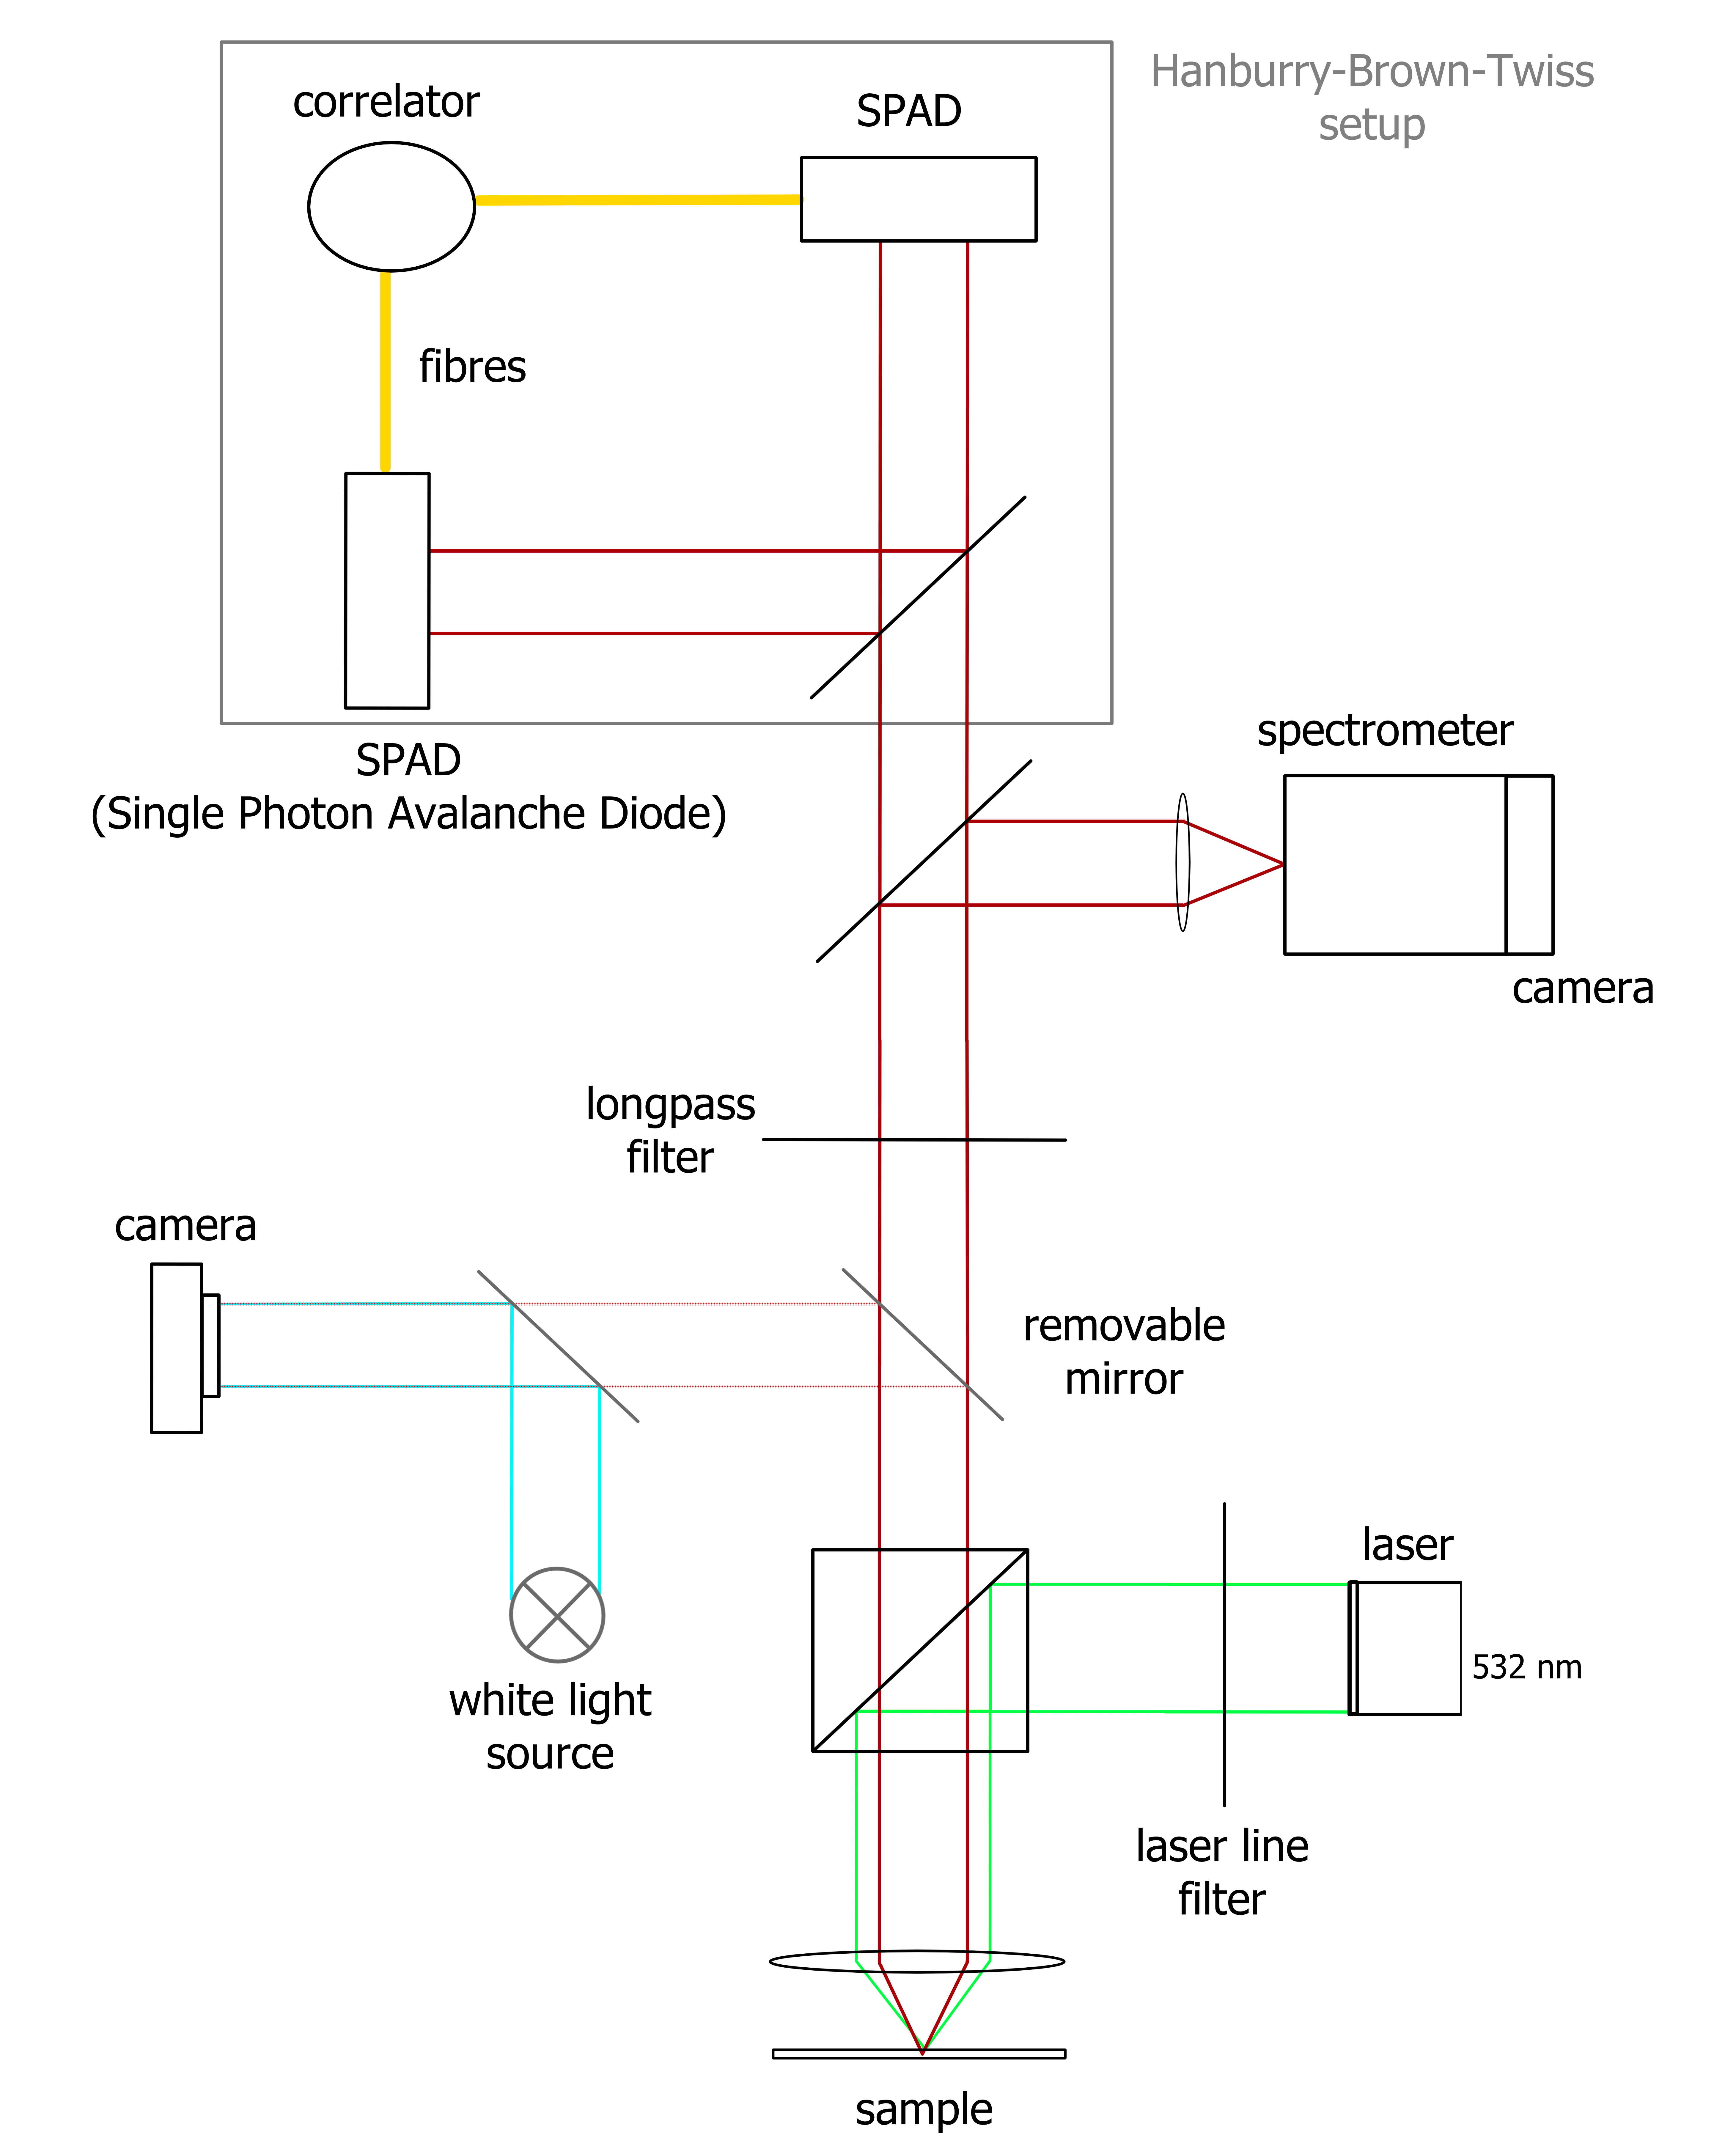
\includegraphics[width=0.6\textwidth]{img/setup2.png}
    \caption{Schematic of the confocal microscope used to record photoluminescence antibunching autocorrelation plots.}
    \label{fig_confocal}
\end{figure}

Hexagonal boron nitride powder on a substrate is viewed through a confocal microscope, which is shown in \cref{fig_confocal}.
For the measurements a laser and a detector is used.
The laser is passed through a laser line filter, to sharpen its energy distribution.
In order to navigate on the sample, a white light source and a camera are used.
Once a promising region is found, the laser and the spectrometer are used, to record spectra at different spots on the sample, until a likely single photon emitter (SPE) is found.
The likely SPE is identified through having a clean spectrum that only contains peaks of one SPE and no other photon sources.

Once a suspected SPE is found, an antibunching measurement is conducted, by replacing the spectrometer with two fibres that split the light into two parts, that are seperately measured with two detectors as described in \cref{sec:theory:spe}.
These measurements are conducted for a series of different excitation laser powers and for each measurement a seperate background measurement is done, by sending the laser immediately onto the detector without passing the sample.

Additionally spectra are also recorded for increasing laser powers. %verwechsele ich laser powers oder ist das doppelt mit dem vorherigen Satz? ->ne, das davor bezieht sich auf Antibunching und hier meine ich die Spektren.

\subsection{Analysis}
\subsubsection{Antibunching}
\label{sec:spe:analysis:antibunch}

In \cref{fig_antibunch_raw} the raw measurement data recorded in the procedure described above is shown.
In the following the measurement of the SPE will be called $S(\tau)$ and the background measurement will be called $B(\tau)$ with $\tau$ the delay measured between the two detectors.
It can be seen, that peaks exist in both measurements.
These stem from reflections in the fibre of the HBT setup.
As these resonances are independent of the sample, the background measurement contains only these resonances and can be used to derive a background corrected signal $\tilde{S} (\tau)$.
If the average number of counts in a bin far away from the dip or any resonances is $I_S$ for the SPE measurement and $I_B$ for the background, the correction can be done as follows:
\begin{equation}
  \tilde{S} (\tau) = S - \frac{I_S}{I_B F} (B-I_B) = S - \frac{I_S}{I_B F} B + I_S
\end{equation}
Here $B-I_B$ gives only the resonance peaks and $\frac{I_S}{I_B}$ renormalizes them from the background measurement to the SPE measurement.
The factor $F$ is added artificially and is manually adjusted for each measurement, as without it the resonance peaks are overestimated causing minima in the corrected signal.
This may be due to the existence of the sample having an effect on the relative intensity of the peaks.
In order to do this the term $\frac{I_S}{I_B F} (B-I_B) + I_S$ is plotted in comparison to the uncorrected signal as shown in \cref{fig_antibunch_background_comp} and $F$ is adjusted, until the resonance peaks match up.
The values used for $F$ lie in the range of \SIrange{1,5}{6}{}.
In \cref{fig_antibunch_raw_corr_comp} the corrected signal $\tilde{S}$ is compared to the raw signal $S$.
Also the delay times are adjusted by an offset of \SI{98,5}{ns}, so that the dip lies at \SI{0}{ns}.
This is necessary due to slightly different travelling time of the signal between the detectors.
Only the part of the measurement close to the dip is shown.


\begin{figure}[H]
    \centering
    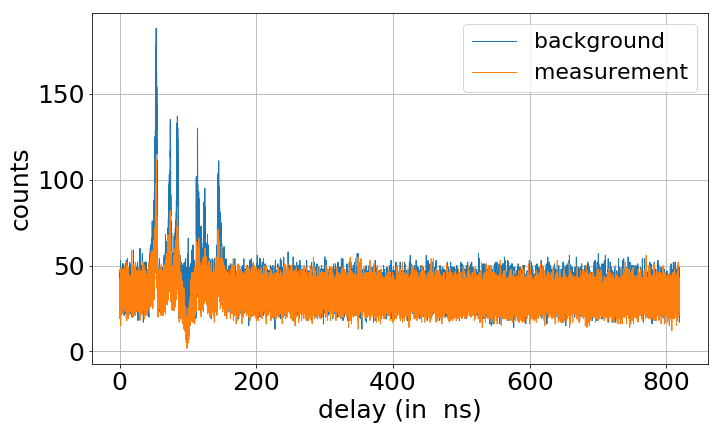
\includegraphics[width=0.7\textwidth]{img/output_t2/antibunch_example_50.0muW.png}
    \caption{Antibunching measurement of hBN and the background measurement as recorded for a laser power of \SI{50}{\micro W}.}
    \label{fig_antibunch_raw}
\end{figure}

\begin{figure}[H]
    \centering
    \begin{subfigure}{0.7\textwidth}
        \centering
        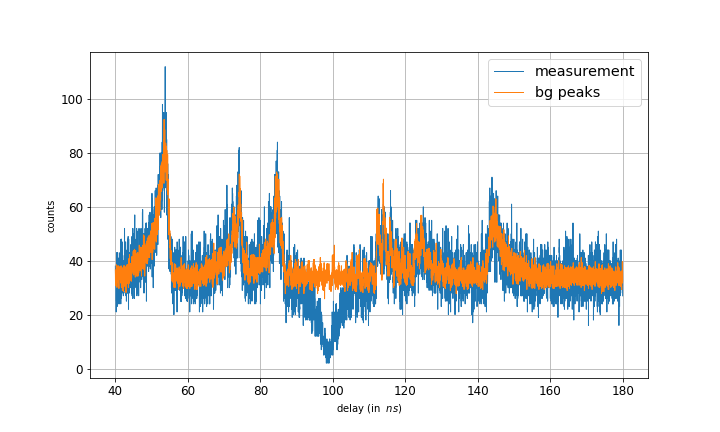
\includegraphics[width=1.0\textwidth]{img/output_t2/50.0muW_bg_peaks.png}
    \caption{}
    \label{fig_antibunch_background_comp}
    \end{subfigure}
    %\hfill
    \begin{subfigure}{0.7\textwidth}
        \centering
        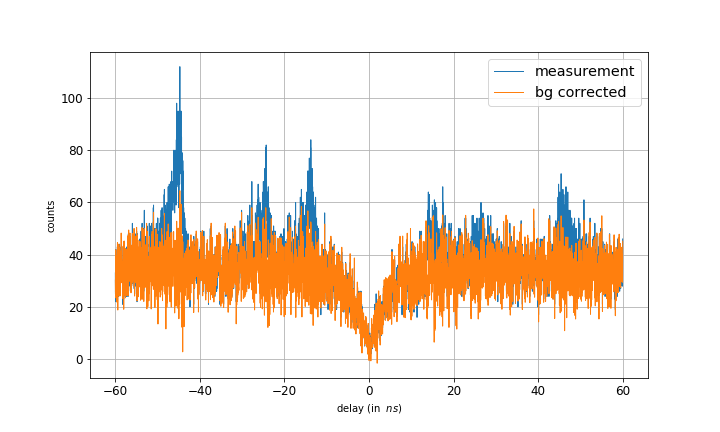
\includegraphics[width=\textwidth]{img/output_t2/50.0muW_bg_vgl.png}
        \caption{}
        \label{fig_antibunch_raw_corr_comp}
    \end{subfigure}
    \caption{a: Antibunching measurement as recorded and compared to the adjusted background signal. b: Antibunching measurement as recorded and compared to the background corrected signal. The laser power is \SI{50}{\micro W}.}
	\label{fig_antibunch_comp}
\end{figure}

This is done for six different powers and shown in \cref{fig_waterfall}.
The individual plots with and without background correction can be seen in \cref{sec:anhang:spe}.

\begin{figure}[H]
    \centering
    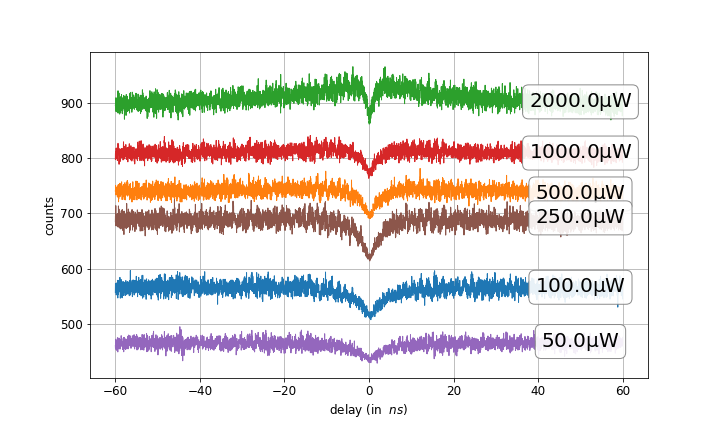
\includegraphics[width=0.9\textwidth]{img/output_t2/massvgl_bgcorr}
    \caption{Background corrected antibunching measurements for different laser powers. A vertical offset has been added to seperate the plots.}
    \label{fig_waterfall}
\end{figure}

These antibunching measurements show that indeed a single photon emitter was found, as they all show a significant dip at a delay between start and stop signal of \SI{0}, because this means that it is at least much less likely that the source emits two photons at once, than at a finite delay.
It can also be seen that for very high laser powers the edges of the signal start to decrease significantly with the absolute value of the delay time.
This can be explained by the fact, that here the photon rate emitted from the laser and thereby from the sample is so high that large delays between start and stop signal become increasingly unlikely independently of the sample.

In order to characterize the behavior of the source at increasing excitation powers, the depth of the dip and the width of the dip at half of its depth is manually read from the charts.
The results are shown in \cref{fig_dip_depth} and \cref{fig_dip_width}.
The depth is normalized by $I_S$ to ensure comparibilty between measurements.
The uncertainties are gauged from the thickness of the noise.
For the power an uncertainty of $1\%$ is assumed.


\begin{figure}[H]
    \centering
    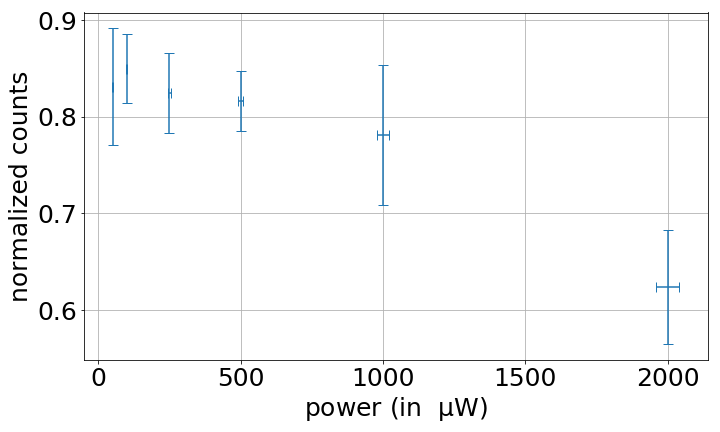
\includegraphics[width=0.7\textwidth]{img/output_t2/dip_depth.png}
    \caption{Depth of the dips in the antibunching measurements plotted against the laser power.}
    \label{fig_dip_depth}
\end{figure}

\begin{figure}[H]
    \centering
    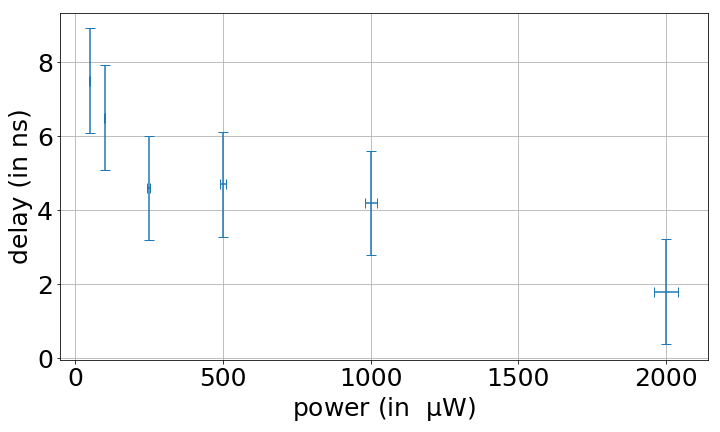
\includegraphics[width=0.7\textwidth]{img/output_t2/dip_width.png}
    \caption{Width of the dips in the antibunching measurements plotted against the laser power.}
    \label{fig_dip_width}
\end{figure}

It can be seen that both the depth and the width decreases with increasing laser power.
For the depth this is explained by the behavior of the avalanche detectors, which show a finite time precision (jitter).
For higher powers, the delay time is reduced and the depth of the dip decreases due to the jitter.

It is also observed that the SPE starts blinking at high powers, disappearing for short periods of time, before reappearing.
This can be explained, by supposing that at this photon rate the emitter reaches periods of saturation in the way that electron-hole pairs are created faster than they can decay, causing periods of time, where there are no excitable electrons available.
%TODO Mail-Antwort

\subsubsection{Spectra and Power efficiency of the SPE}

In \cref{fig_spe_spectrum_example} an example of the recorded spectra is shown.
A constant background has been substracted, so that there are no counts at high wavelengths.
The large peak corresponds to the main zero-phonon decay of an exciton, while to the right two peaks of the one-phonon decay and even two very small peaks of the two-phonon decay can be seen.
For the one-phonon decay both peaks belong to longitudinal phonons.
Though for the two-phonon decay three combinations are possible (longitudinal-longitudinal, longitudinal-transverse, transverse-transverse), only two small peaks can be seen in the spectrum, possibly because the energy difference between two of these combinations isn't high enough to allow seperation at these low count rates.
%vmtl optisch, aber kp
The small peak at \SI{532}{nm} is caused by the reflection of the laser itself, as this is its wavelength.
It is small, because most of it gets filtered out by the longpass filter.

\begin{figure}[H]
    \centering
    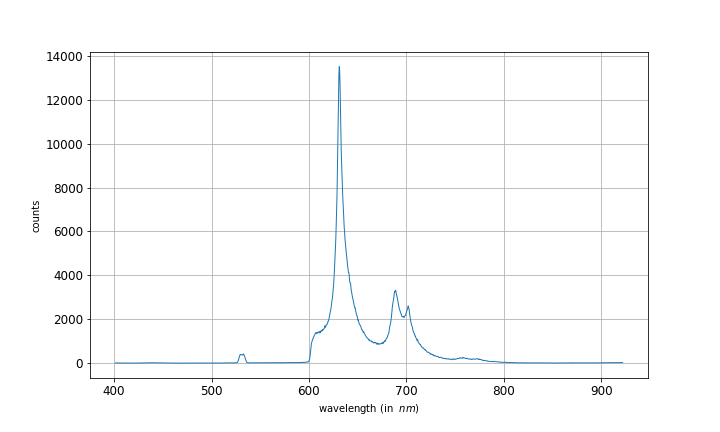
\includegraphics[width=0.7\textwidth]{img/output_t2/spektrum_example_bgcorr_200.0muW.png}
    \caption{Recorded Spectrum of the observed single photon emitter at a laser power of \SI{200}{\micro W}. A constant background has been substracted.}
    \label{fig_spe_spectrum_example}
\end{figure}

In order to observe the behavior of the SPE at increasing laser powers, in \cref{fig_spe_integrals} each spectrum has been integrated and normalized over the time that the spectrum was recorded over. %theoretisch hätte man hier den Laserpeak rauslassen sollen, aber macht auch keinen großen Unterschied.
It can be seen, that the output increases mostly linearly with the power meaning that the efficiency is approximately constant.
It would be expected that at higher powers the SPE approaches saturation, causing the efficiency to go down and the increase in output photons to be reduced.
This could not be seen, as the observed SPE died at \SI{450}{\micro W}.
%warum nicht linear bei kleinen Leistungen?

\begin{figure}[H]
    \centering
    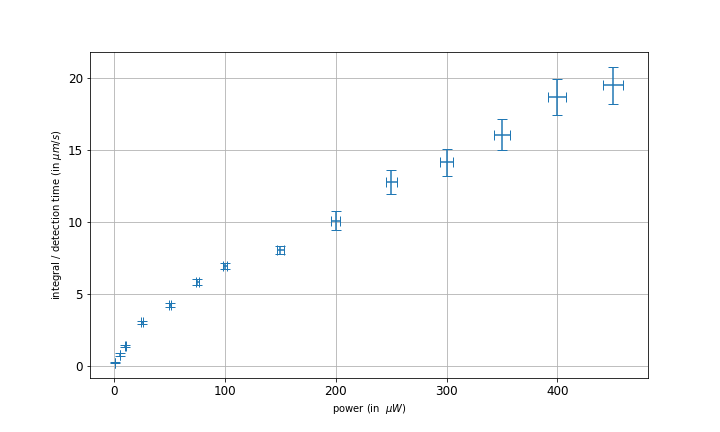
\includegraphics[width=0.7\textwidth]{img/output_t2/integrals.png}
    \caption{Integrated spectra of the SPE normalized by the detection time at different laser powers.}
    \label{fig_spe_integrals}
\end{figure}
